
\chapter{Strengthening SSH Password Authentication with SFE}


\section{SSH Protocol Overview}

SSH is an application originally designed as an alternative to telnet
for interactive sessions with confidentiality, authentication, and
integrity. In the years since it was first introduced, it has gained
many features and can now serve as a secure transport layer underneath
many other insecure protocols. Version 1 of the SSH protocol was essentially
undocumented, but version 2, which is commonly used today, is an IETF
standard. From here on, all references to the SSH protocol refer to
version 2 unless otherwise specified.

The SSH protocol is defined in terms of layers, much like the OSI
networking stack. Each layer is defined in terms of messages from
the underlying layer. The lowest level is an application packet based
transport protocol that is layered on top of TCP. All SSH messages
of the higher layers are sent as packets. This packet protocol is
known as the SSH transport layer protocol and is defined in \cite{rfc4253}.
Figure \ref{fig:ssh-overview} shows the hierarchy of the ssh protocol
layers discussed here. The SSH transport layer also handles the server
key authentication, encryption, and integrity of a session. 

\begin{center}
%
\begin{figure}
\begin{centering}
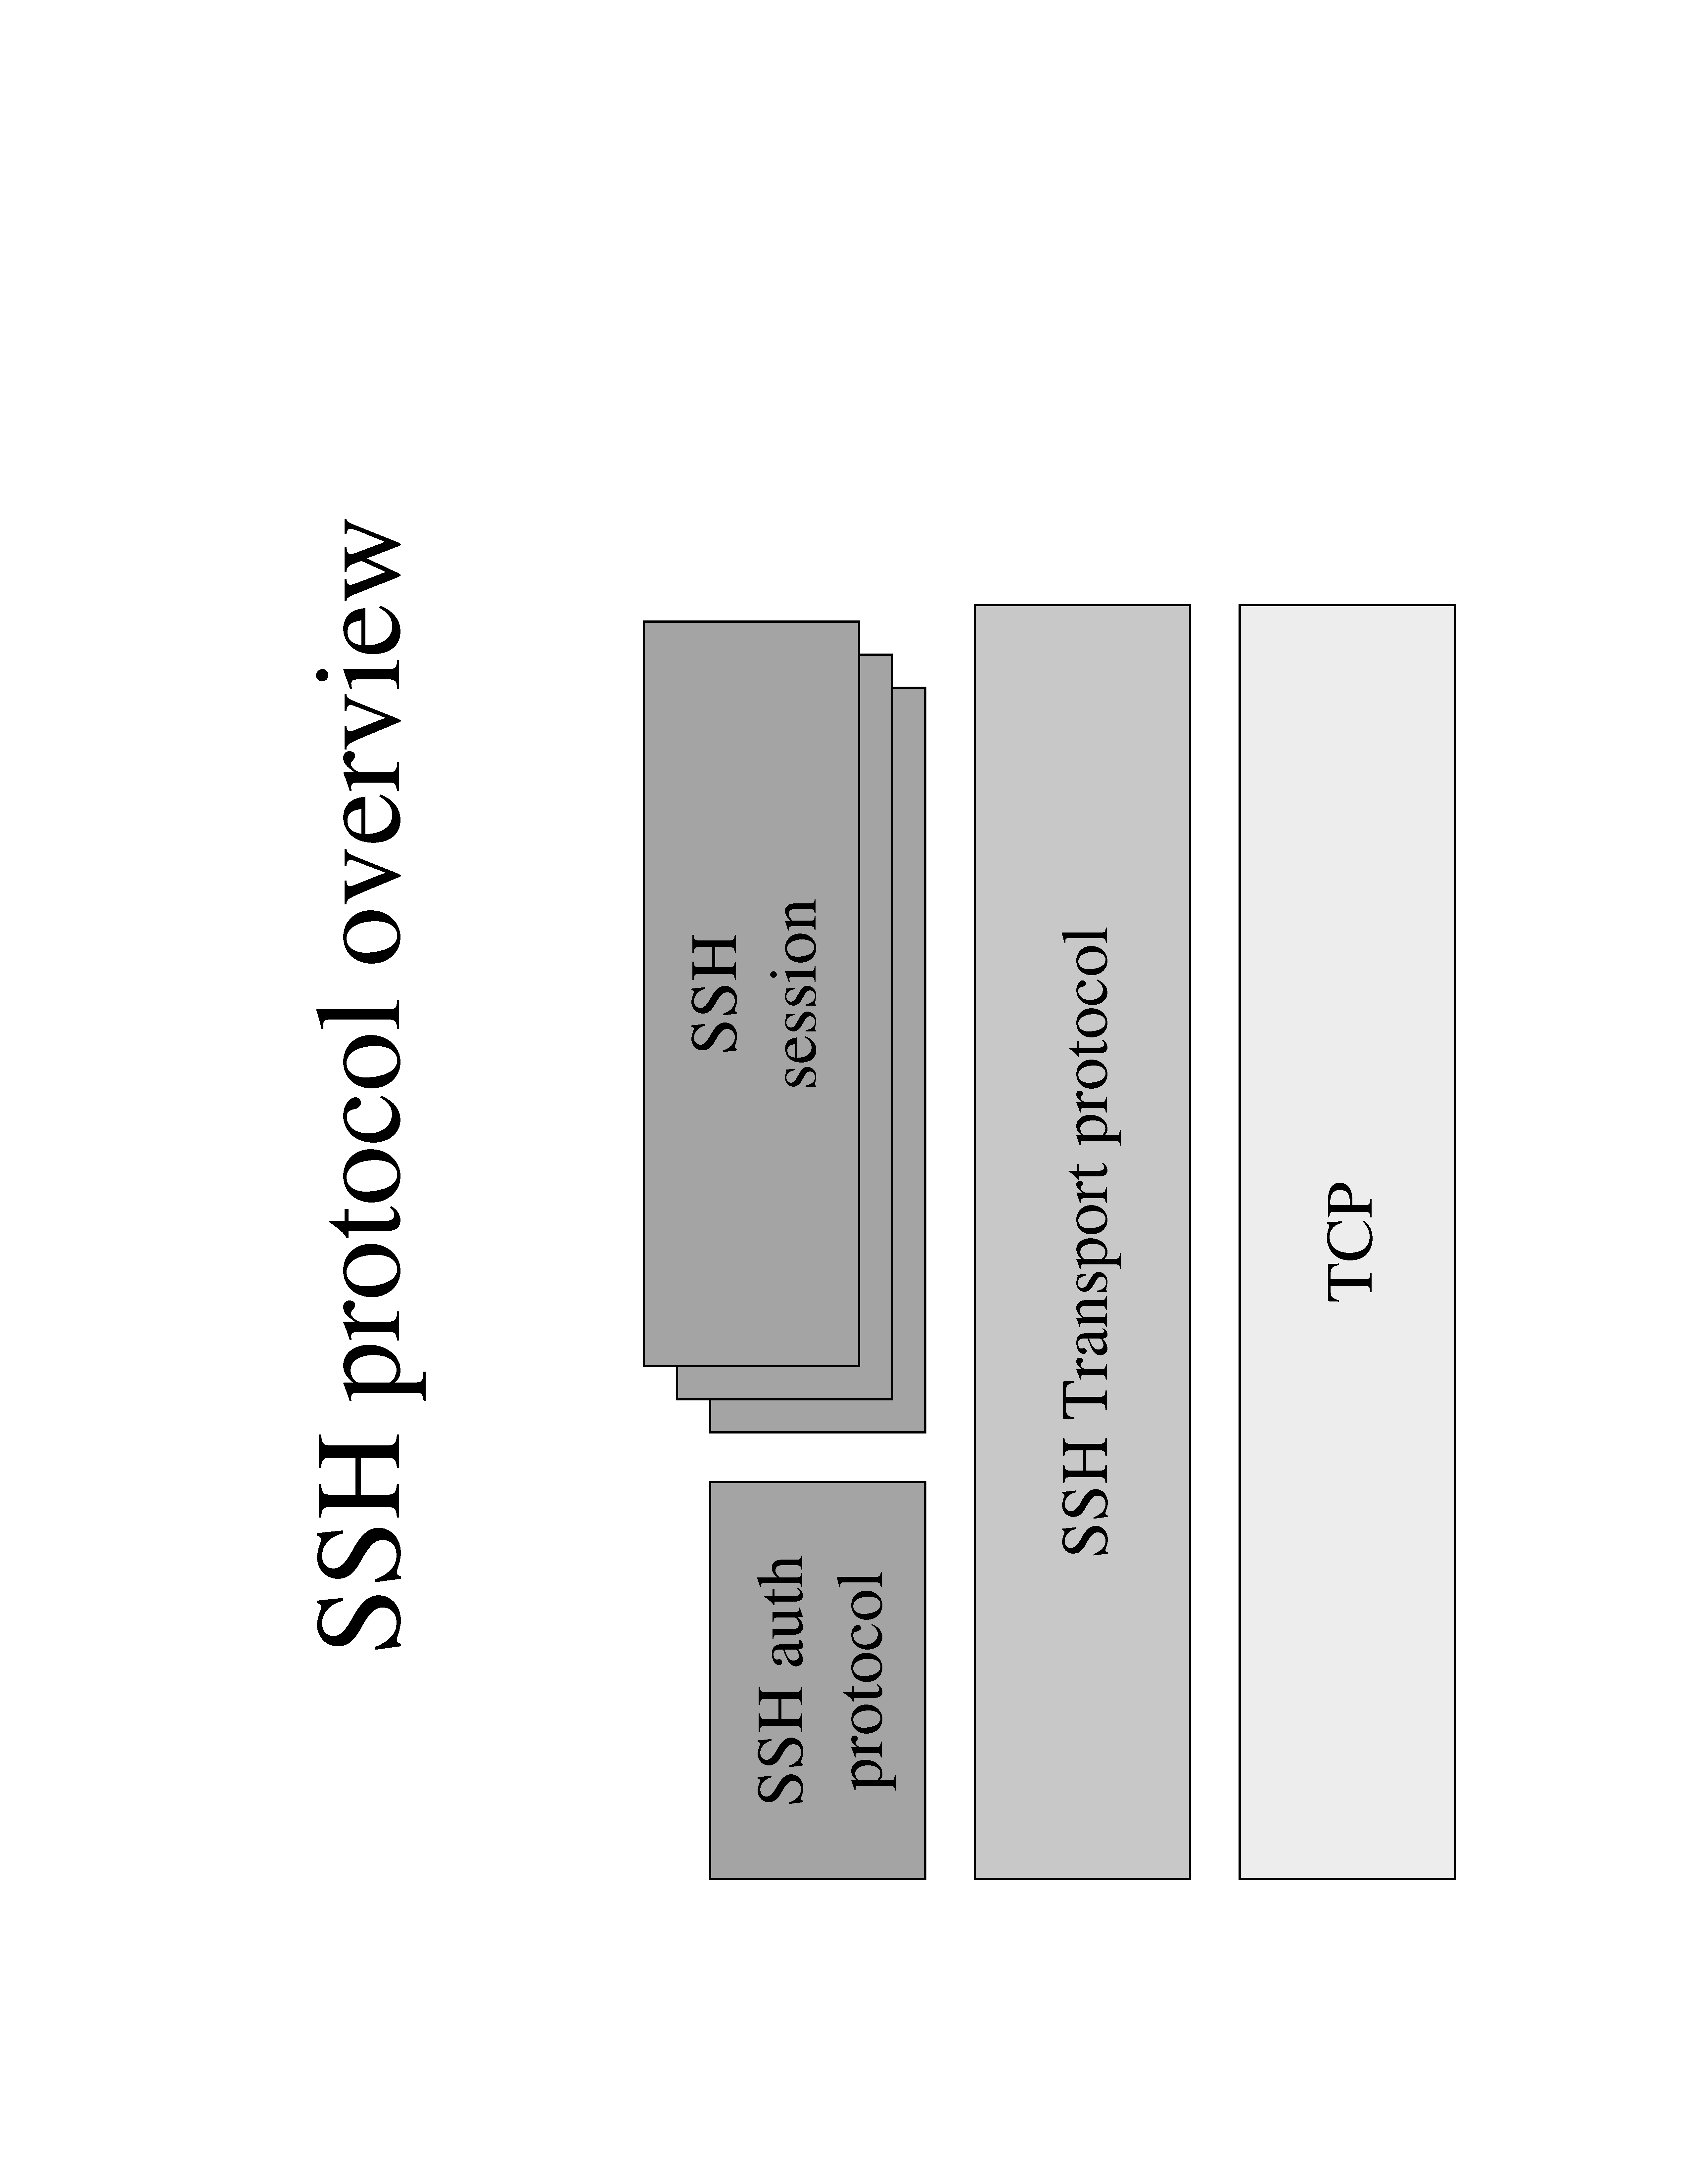
\includegraphics[clip,scale=0.4,angle=270]{ssh_overview}
\par\end{centering}

\caption{\label{fig:ssh-overview} protocol hierarchy}

\end{figure}

\par\end{center}


\subsection{Session Initialization}

During the initial handshake, the hosts perform a key exchange and
the client validates the server key, and there is negotiation for
an initial set of cryptographic algorithms (cipher, HMAC) that will
used for the session. An overview of the handshake messages are shown
in figure \ref{fig:ssh-init}. The steps of the protocol are as follows.
Refer to figure \ref{fig:ssh2-init} for details.
\begin{enumerate}
\item The SSH server sends a string of the form {}``SSH-2.0-\emph{software}''.
The \emph{software} string identifies the particular client or server.
(as a variation, it may also send SSH-1.99-\emph{software''} to indicate
protocol version 1 compatibility) For example, the OpenSSH 4.5 software
sends {}``SSH-1.99-OpenSSH\_4.5''. If the client does not understand
the protocol version, it disconnects, otherwise it sends a similar
string to the server. After these strings are sent, all traffic uses
the binary packet protocol shown in figure  \ref{fig:ssh-packet}.\\
%
\begin{figure}
\begin{centering}
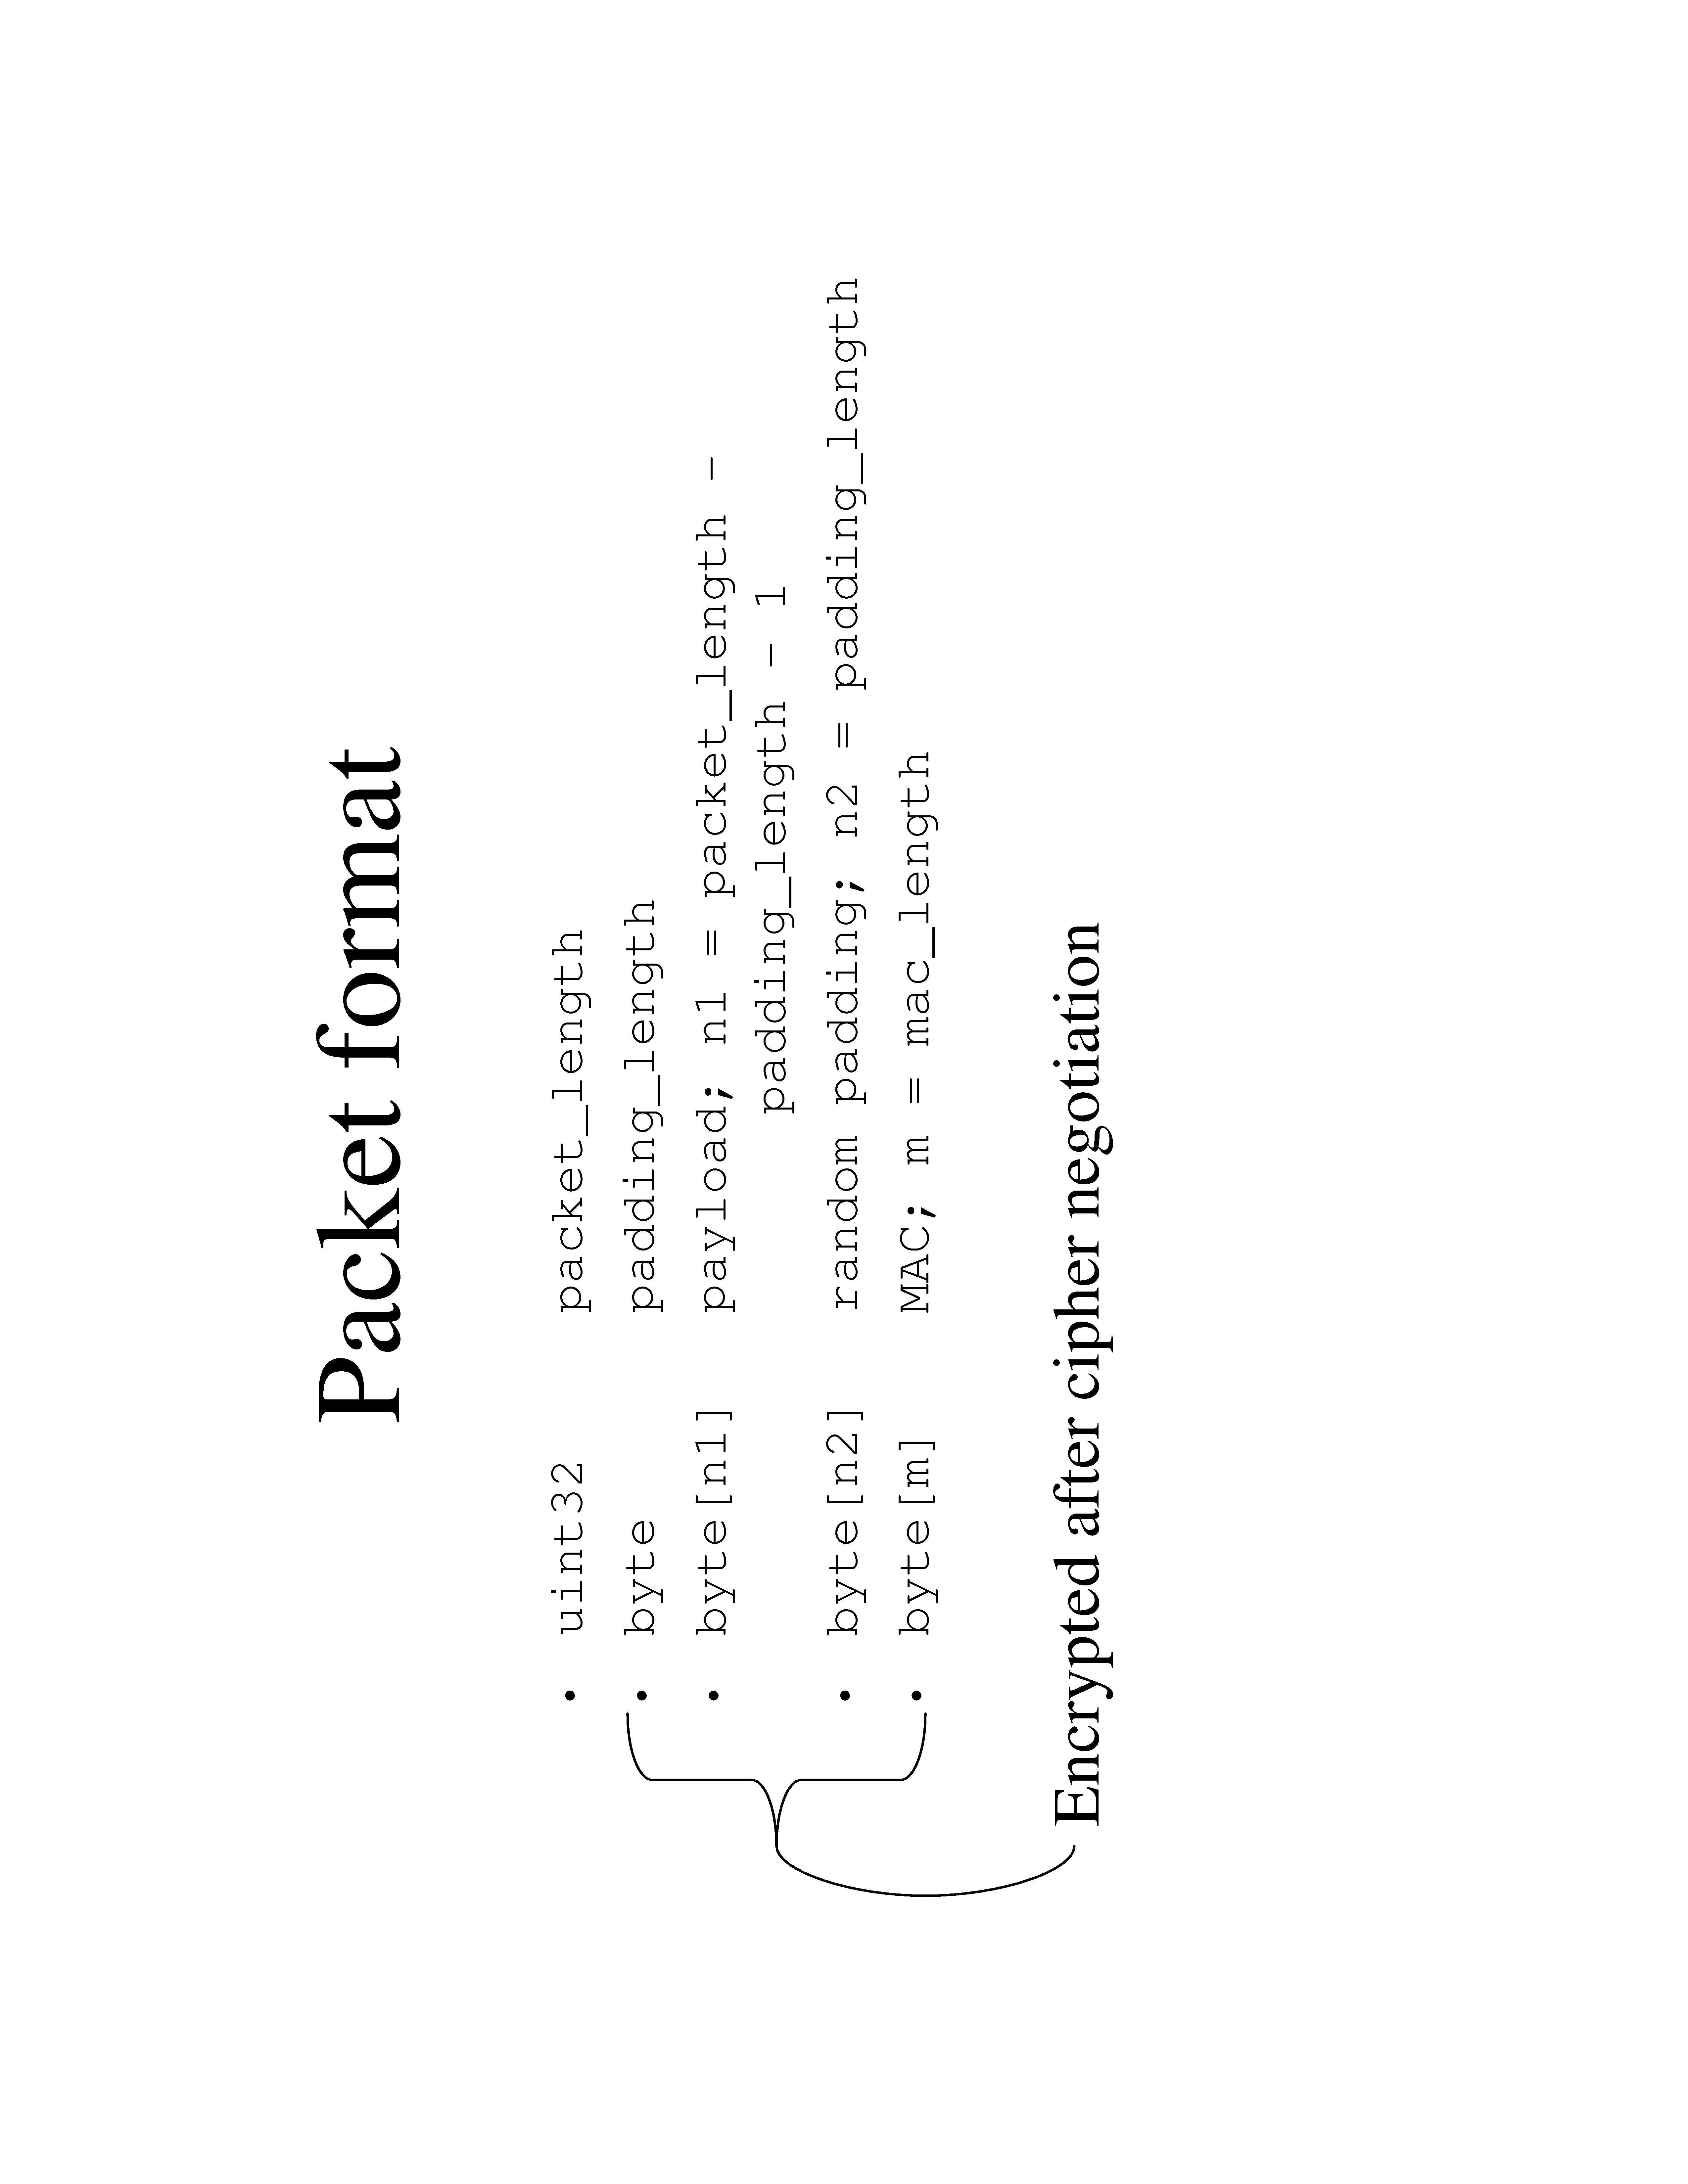
\includegraphics[clip,scale=0.4,angle=270]{ssh_packet}
\par\end{centering}

\caption{\label{fig:ssh-packet} binary packet structure}

\end{figure}

\item Each party sends an SSH\_MSG\_KEXINIT message to begin the key exchange.
This message includes a list of supported ciphers, HMAC algorithms,
compression algorithms, and key exchange algorithms, ranked by preference.
For each algorithm, the parties choose the highest preference algorithm
of the client, which is also supported by the server. If one of the
algorithm lists has no algorithm in common, the connection is terminated.
The format of the SSH\_MSG\_KEXINIT message are as follows:

\begin{lyxcode}
~~~~~~byte~~~~~~~~~SSH\_MSG\_KEXINIT

~~~~~~byte{[}16{]}~~~~~cookie~(random~bytes)

~~~~~~name-list~~~~kex\_algorithms

~~~~~~name-list~~~~server\_host\_key\_algorithms

~~~~~~name-list~~~~encryption\_algorithms\_client\_to\_server

~~~~~~name-list~~~~encryption\_algorithms\_server\_to\_client

~~~~~~name-list~~~~mac\_algorithms\_client\_to\_server

~~~~~~name-list~~~~mac\_algorithms\_server\_to\_client

~~~~~~name-list~~~~compression\_algorithms\_client\_to\_server

~~~~~~name-list~~~~compression\_algorithms\_server\_to\_client

~~~~~~name-list~~~~languages\_client\_to\_server

~~~~~~name-list~~~~languages\_server\_to\_client

~~~~~~boolean~~~~~~first\_kex\_packet\_follows

~~~~~~uint32~~~~~~~0~(reserved~for~future~extension)
\end{lyxcode}
%
\begin{figure}
\begin{centering}
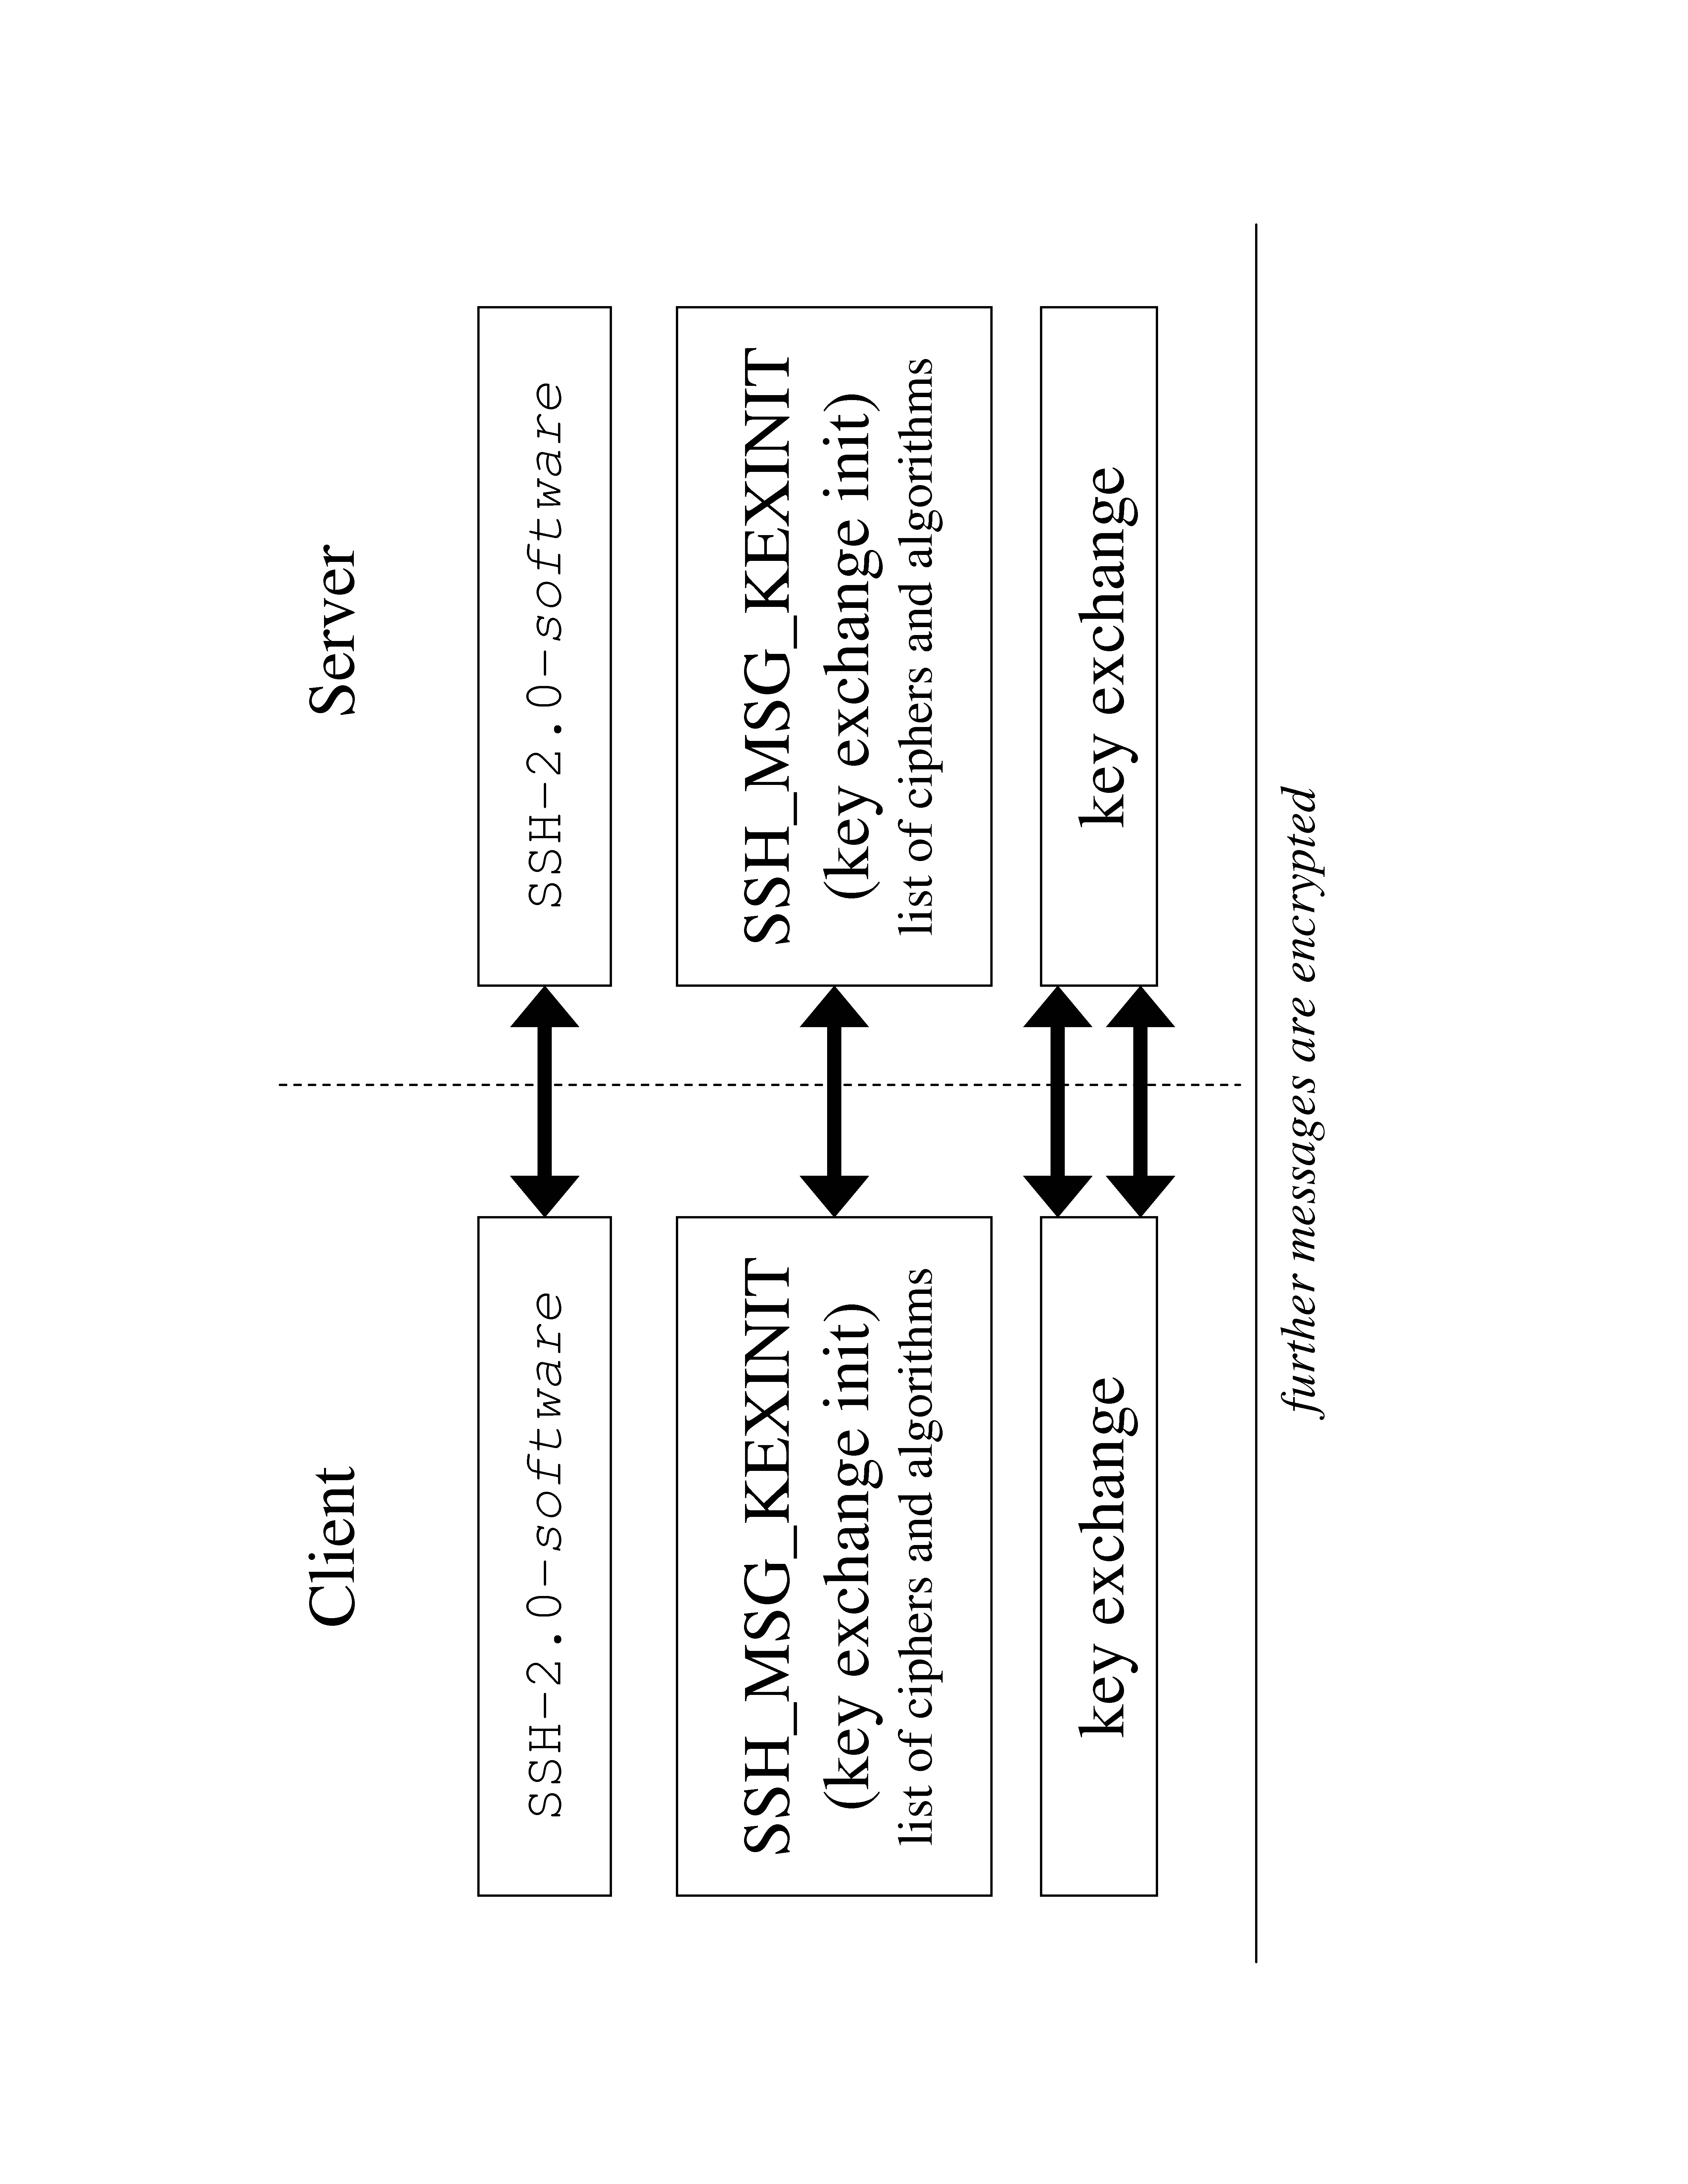
\includegraphics[clip,scale=0.4,angle=270]{ssh_init}
\par\end{centering}

\caption{\label{fig:ssh-init} connection handshake protocol}

\end{figure}


%
\begin{figure}
\begin{centering}
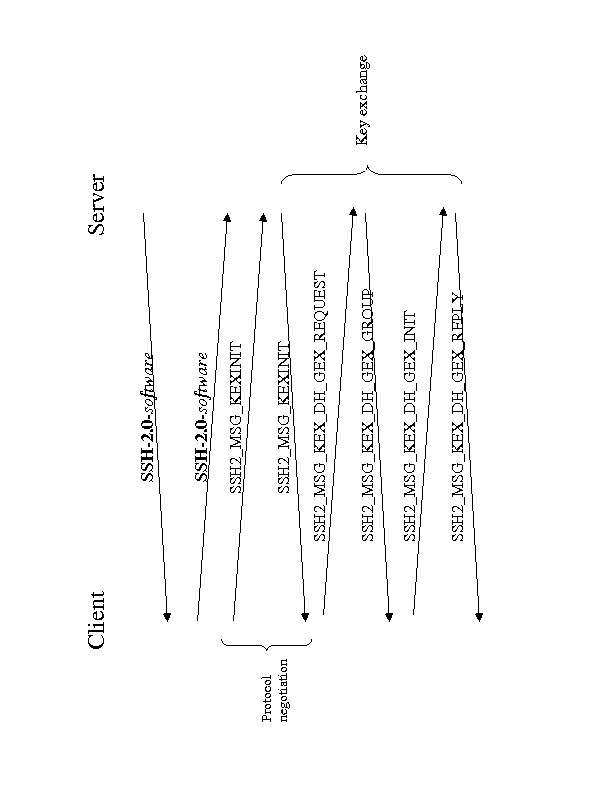
\includegraphics[clip,scale=0.4,angle=270]{ssh2_p1}
\par\end{centering}

\caption{\label{fig:ssh2-init} connection handshake protocol}

\end{figure}


\item Following the handshake, the key exchange protocol is performed. The
specific algorithm used to do the key exchange is negotiated in the
previous step. The original SSH2 specification included a single Diffie-Hellman
group defined in \cite{rfc4253}. A newer and more flexible key exchange
algorithm is defined in \cite{rfc4419}. The details of key exchange
will not be discussed further. After the key exchange is complete,
all of the data in the SSH stream is encrypted using the negotiated
cipher and key. Specifically, the sequence of packets, excluding the
packet size header, shown in \ref{fig:ssh-packet} is a single stream
of plaintext encrypted by the cipher.
\end{enumerate}
At this point, the protocol handshake is complete and the client may
initiate arbitrary sub-protocols of SSH. Typically, however, the client
will begin the client authentication protocol, as most servers require
authentication before allowing other services to be provided.


\subsection{Client Authentication}

When the initial handshake is complete, the client has verified the
server key, if possible, but the client has not yet authenticated
to the server. The SSH auth protocol can be initiated to perform this,
and is defined by \cite{rfc4252}. The auth protocol is flexible.
The SSH standard describes several standard methods of authentication,
such as password and public-key, arbitrary additional vendor or site-specific
authentication methods can be added.

To authenticate, the client chooses an authentication protocol. Here,
I will consider two standard authentication types: {}``password''
and {}``keyboard-interactive''. The difference between these methods
is that {}``password'' allows only a single packet with a user name
and password combination, whereas {}``keyboard-interactive'' allows
the server to send arbitrary prompts and wait for responses. This
is suitable for multi-factor authentication. For example, using {}``keyboard-interactive''
the server could first ask for a password, and then follow up with
a series of challenge questions, and a random string from a secure
token.

The messages used in password authentication are shown in Figure \ref{fig:ssh-auth}.
For the purposes of this discussion, we will assume the client is
using the {}``password'' authentication method. The steps of this
authentication are as follows:
\begin{enumerate}
\item The client sends the username and password to the server in an SSH\_MSG\_USERAUTH\_REQUEST
message. The format of this message is:

\begin{lyxcode}
~~~~~~byte~~~~~~SSH\_MSG\_USERAUTH\_REQUEST

~~~~~~string~~~~user~name~in~ISO-10646~UTF-8~encoding~{[}RFC3629{]}

~~~~~~string~~~~\textquotedbl{}password\textquotedbl{}

~~~~~~boolean~~~FALSE

~~~~~~string~~~~plaintext~password~in~ISO-10646~UTF-8~encoding~


\end{lyxcode}
\item If the server does not support the {}``password'' method chosen,
or the password is incorrect, the server will respond with an SSH\_MSG\_USERAUTH\_FAILURE
message. If the password is correct, the server sends a SSH\_MSG\_USERAUTH\_SUCCESS
message, and the client may begin requesting services. (The server
may also send a SSH\_MSG\_USERAUTH\_BANNER packet to communicate information
directly to the user. It is analogous to the /etc/issue file used
in standard Unix systems to display a message at a login prompt)
\end{enumerate}
%
\begin{figure}
\begin{centering}
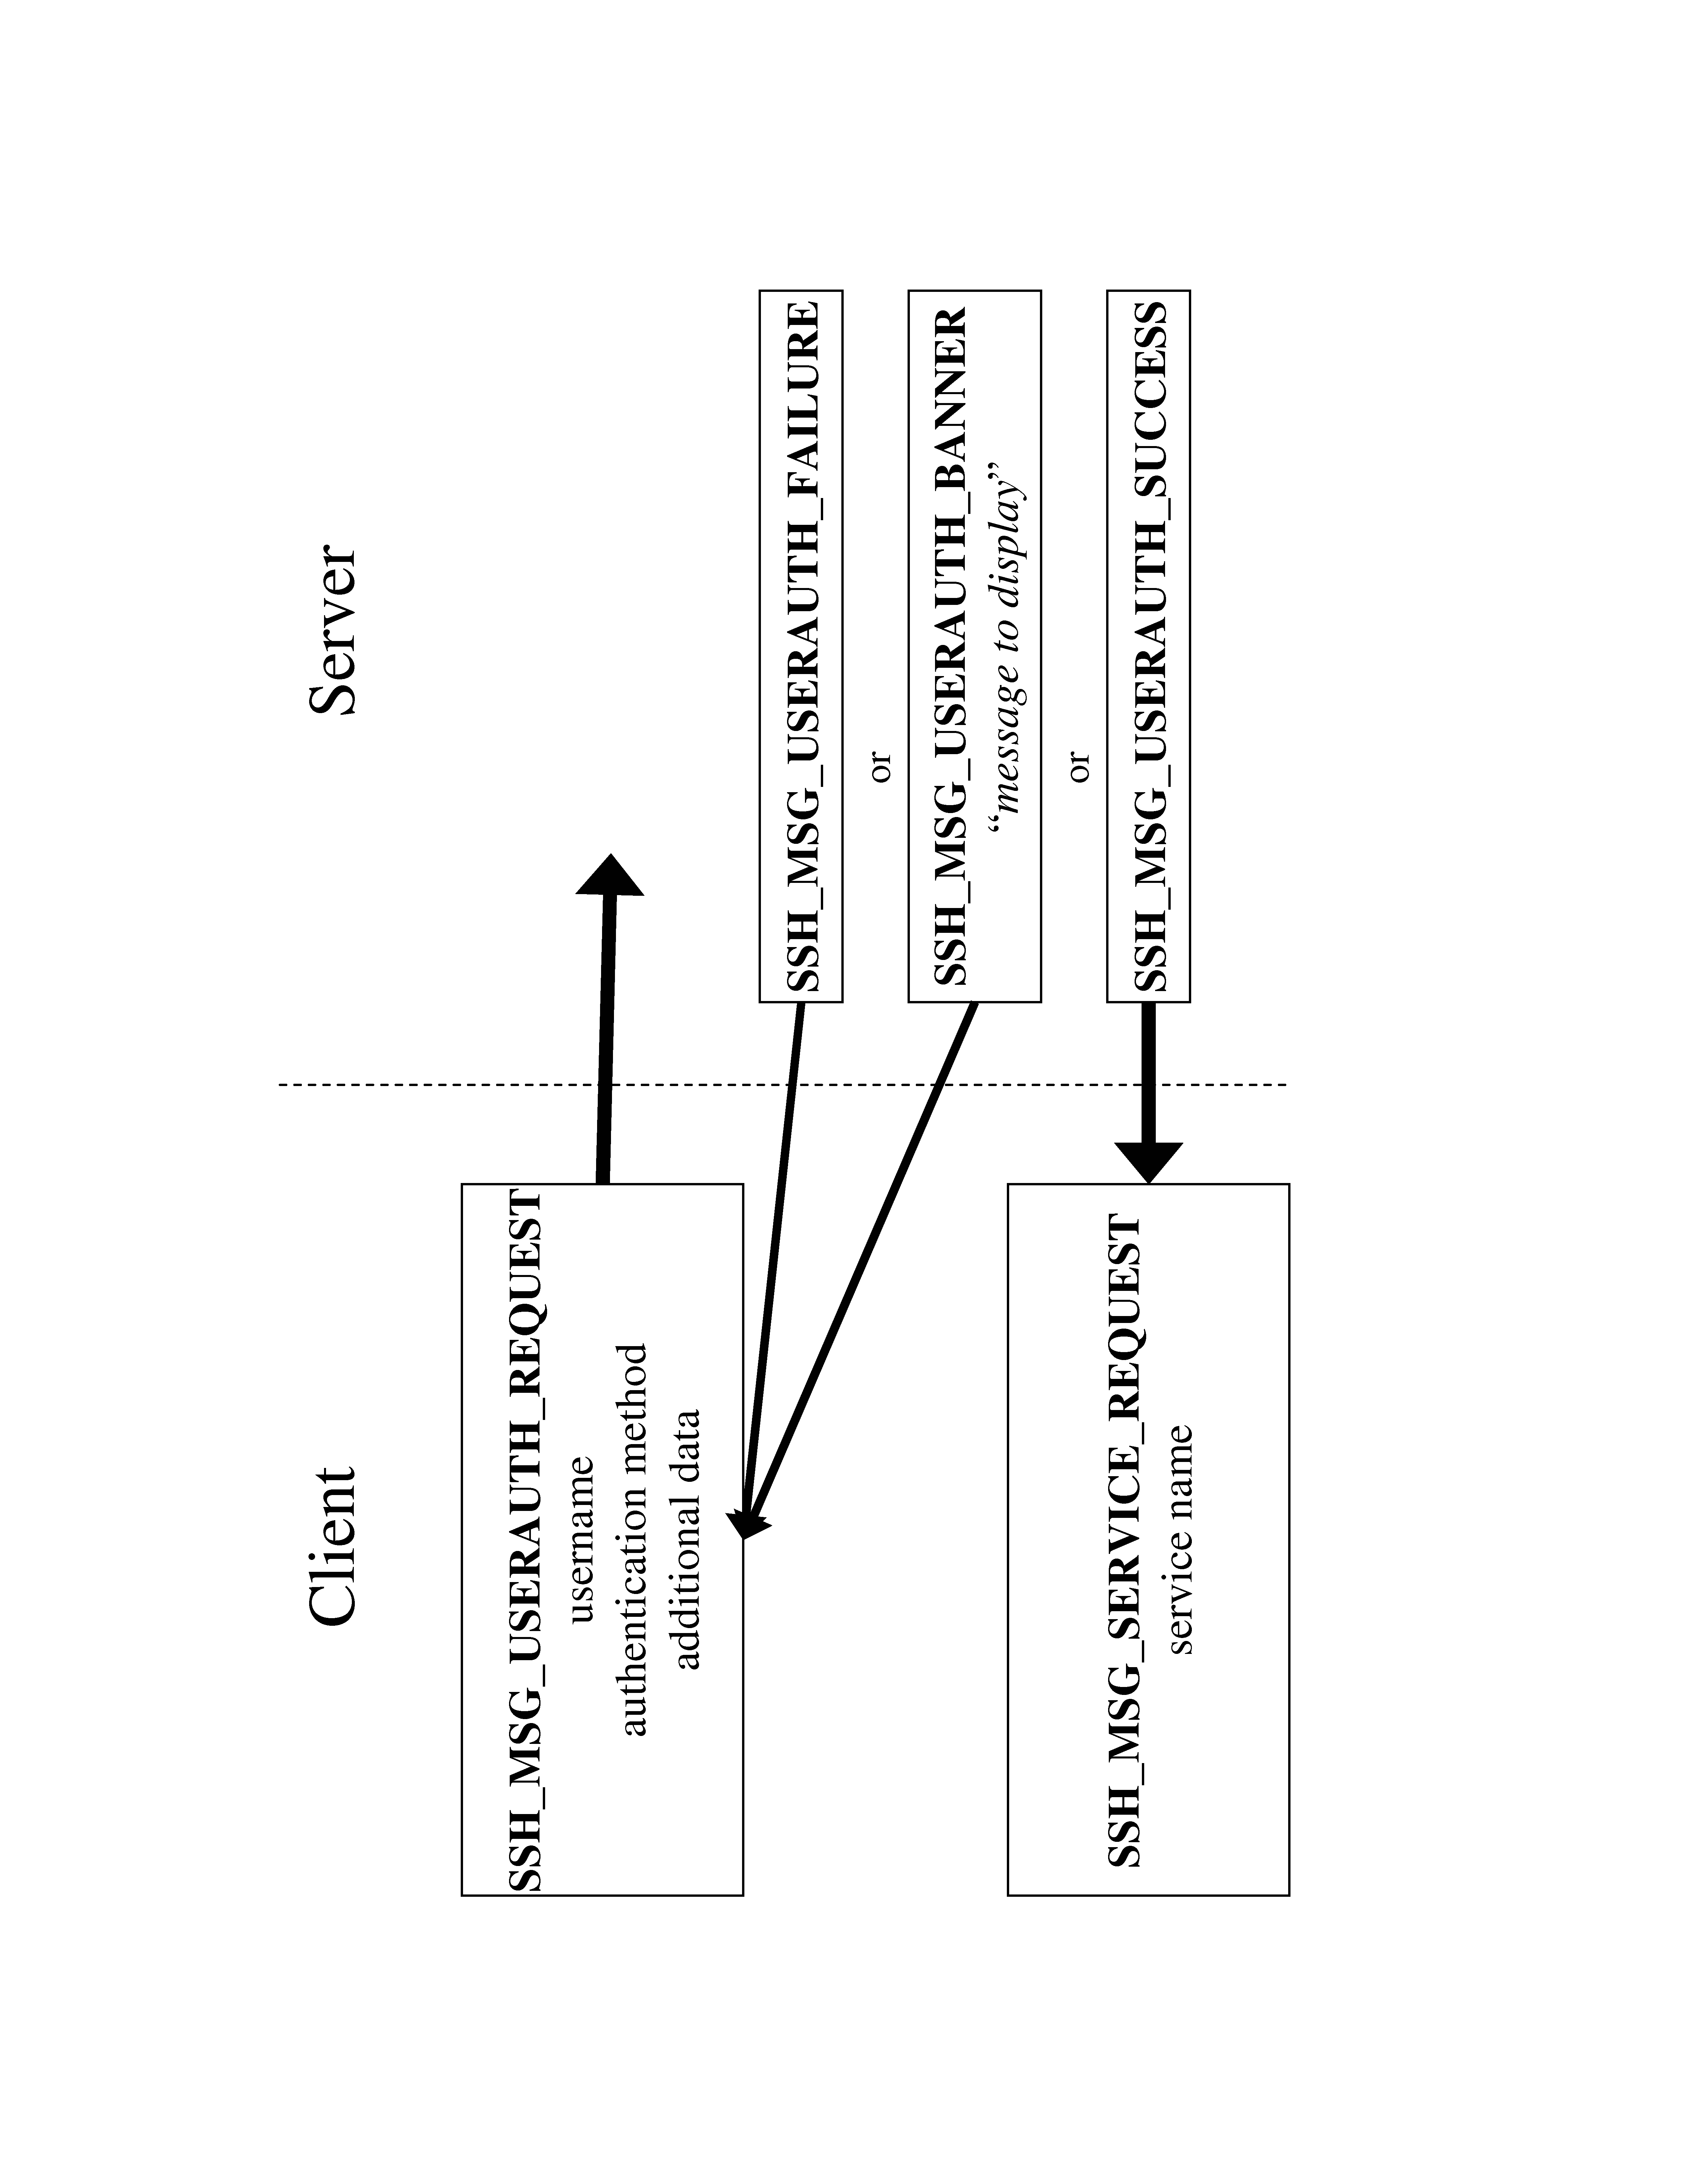
\includegraphics[clip,scale=0.4,angle=270]{ssh_auth}
\par\end{centering}

\caption{\label{fig:ssh-auth} authentication protocol messages}

\end{figure}


It is easy to see that the password is sent directly from the client
to the server in a packet. Thus, the only protection from eavesdroppers
is the encryption applied at the SSH transport layer. There is no
protection of the client's authentication credentials from the server
itself, so if the server is malicious or has been compromised, an
attacker will learn everything the client sends, and can potentially
impersonate the client at another time.


\section{Man in the Middle Attack \label{sub:Man-in-the-Middle}}

As mentioned in the previous section, the SSH protocol is vulnerable
to password compromise. An attacker can exploit the insecurity of
password transmission by mounting a \emph{man in the middle} (MITM)
attack. Although the protocol does provide some protection against
MITM in the form of host key authentication, there are at least three
ways in which an attacker can thwart this protection:
\begin{enumerate}
\item If the attacker manages to steal the host key, then the attacker can
successfully impersonate the server without detection. There is no
other means for the client to authenticate the server.
\item If the client does not know the server's host key, then the host cannot
be authenticated unless the client has an alternative trusted channel
to validate the host key. The following message is typically displayed
by the OpenSSH client when connecting to a server with an unknown
key\\
%
\begin{minipage}[t]{1\columnwidth}%
\begin{lyxcode}


The~authenticity~of~host~'prospero~(128.105.121.27)'~can't~be~established.

RSA~key~fingerprint~is~3f:76:22:43:c2:03:b9:71:b0:31:ce:87:37:45:cb:02.~

Are~you~sure~you~want~to~continue~connecting~(yes/no)?
\end{lyxcode}
%
\end{minipage}\\

\item Practically speaking, it may be inconvenient for a user to authenticate
the server using this message and make a correct decision. It is easy
to imagine a user simply answering yes in order to bypass the inconvenience. 
\item Even if the client does know the server's key, there is no guarantee
that a user would refuse to connect even if the authentication fails.
For example, the user might think the server key changed for a non-malicious
reason such as an operating system upgrade where the administrator
forgot to backup the old key.
\end{enumerate}
This vulnerability can be mitigated by using additional secrets which
are shared between the client and server. A password is a typical
example of a convenient shared secret in common use today. Typically,
a password is considered only as a means of authenticating a client
to a server, but with special protocols a password can also be used
for simultaneous mutual authentication in a way that is secure, and
does not compromise the password if the server is malicious. Such
protocols are known as \emph{shared password and key authentication}
(SPAKA).

It is important to note that a {}``password'' need not be a constant
string that the user remembers over a long period of time, it can
be any string that serves as a mutual authenticator. For example,
secure ID tokens that display constantly changing strings, time synchronized
with the server, are considered to be a more secure alternative to
traditional passwords, such alternatives are readily usable in SPAKA
protocols.


\section{SPAKA}

\emph{Secure Password and Key Authentication} (SPAKA) is a class of
authentication protocols first described in \cite{bellovin92}. SPAKA
protocols are designed to guarantee confidentiality of secrets even
against active adversaries. There have been various SPAKA protocols
proposed in the literature with varying properties. A recent SPAKA
protocol is presented in \cite{brainard03}. In this protocol, the
user's password $P$ is hashed using a hash function $Q=f(P)$, and
$Q$ is split into two shares: $Q_{1}$ and $Q_{2}$. The value of
$Q$, and therefore $P$, can not be derived from either of the two
shares alone, and each share is stored on a separate server. To perform
the protocol, the client splits $f(P)$ into different shares $Q_{1}'$
and $Q_{2}'$, and sends these values to the servers. The servers
then perform an evaluation protocol to determine if $Q_{1}\oplus Q_{1}'=Q_{2}\oplus Q_{2}'$.
The equality test is obfuscated using a variant of a Diffie-Hellman
key exchange, designed to succeed if and only if the equality is true.




\section{SPAKA using SFE\label{sub:SPAKA-using-SFE}}

The design of protocols such as \cite{brainard03} suggests that SFE
can be applied generally to the SPAKA problem. Here, I propose a general
SPAKA construction based on SFE.

Let $X$ be the user's password.

Let $Y=H(X)$ be a hash of $X$

Let $C$ be the client and $S$ be the server. $C$ and $S$ participate
in a secure evaluation of the following function $f$, where $C$
provides input $X$ and $S$ provides input $Y$. $C$ and $S$ both
receive the same output from $f$, which is a single bit.

$f(X,Y)=\left(Y=H\left(X\right)\right)$

If the value of the function is $false$ then the mutual authentication
fails, otherwise the mutual authentication succeeds.

If $f$ is evaluated securely, then $C$ and $S$ are guaranteed not
to learn any information about the computation except for the single
bit of output. 

This SPAKA protocol effectively solves the man-in-the-middle problem.
Suppose the adversary, Eve, poses as the server when communicating
with the client. Eve will be unable to supply the correct value of
$Y$ as input to the function except with negligible probability.
As a result, the output of $F(X,Y)$ will be $false$, and the client
will know the authentication has failed. Due to the security properties
of SFE, it is also guaranteed that Eve will learn no other useful
information from the evaluation. Therefore, the MITM attack described
in section \ref{sub:Man-in-the-Middle} will not succeed. We will
use a secure evaluation protocol that is secure under the malicious
threat model (see section \ref{sub:Threat-Models}) to ensure that
Eve can not attack the protocol itself.

In addition, the use of secure function evaluation has practical advantages.
In comparison to multi-server protocols such as \cite{brainard03},
communication is limited only to the server and client. Because any
hash function $H$ can be automatically compiled into a secure circuit,
this technique can be used as a drop-in replacement into any existing
authentication system, without rehashing or modifying the password
database. I propose to implement this protocol in the standard OpenSSH
software, measure the performance, and make the implementation available
in hopes this will lead to a more secure SSH becoming common use.

%
\begin{comment}
\begin{enumerate}
\item Practical SSH paper
\item New protocol paper
\item Theoretical paper
\item Graduate!!!
\end{enumerate}

\end{comment}
{}

%
\begin{comment}
\bibliographystyle{plain}
\bibliography{somesh,ssh}

\end{comment}
{}
